\chapter{Bundle adjustment}
\label{ch:ba}

Bundle adjustment (BA) is the problem of Chapter~\ref{ch:slam} written
for a camera: find the poses and the 3D points that best explain every
observation in every image. Its name comes from photogrammetry, where
the ``bundles'' of rays from each camera are adjusted until they meet
the points. Chapter~\ref{ch:nls} already contains everything needed to
solve it in principle. In practice, a few thousand points make the
normal equations far too large to solve naively, and what makes BA
practical is a single piece of linear algebra: eliminating the points
first, by the Schur complement. This chapter derives it, deals with the
gauge, extracts uncertainties from the same computation, and then fixes
the flaw that Chapter~\ref{ch:vo} uncovered in our VO: keyframe map
points treated as exact.

\section{The problem}

\begin{definition}{Bundle adjustment}{ba}
Given cameras $T_i=T_{wc_i}$, $i=1,\dots,m$, points $\vect{X}_j\in\R^3$,
$j=1,\dots,n$, and an observation $\z_{ij}$ for every pair in a set
$\mathcal{O}$ (pixel or stereo measurement), minimise
\[
F=\tfrac12\sum_{(i,j)\in\mathcal{O}}\rho\bigl(\norm{\vect{r}_{ij}}^2
\bigr),\qquad \vect{r}_{ij}=\frac{\z_{ij}-h(T_i,\vect{X}_j)}{\sigma},
\]
over $(T_1,\dots,T_m,\vect{X}_1,\dots,\vect{X}_n)$, the cameras being
updated by right perturbations $\bxi_i\in\R^6$ and the points additively.
\end{definition}

The Jacobian of each residual has two non-zero blocks:
$A_{ij}=\partial\vect{r}_{ij}/\partial\bxi_i$ and
$B_{ij}=\partial\vect{r}_{ij}/\partial\vect{X}_j$, given by
\cref{prop:projjac} (or its stereo version) times $-1/\sigma$. With a
robust kernel, the IRLS weights of \cref{prop:irls} multiply both.

\section{The structure of the normal equations}

\begin{proposition}{The arrowhead}{arrow}
Order the unknowns as $(\bxi_1,\dots,\bxi_m,\vect{X}_1,\dots,\vect{X}_n)$.
The Gauss--Newton matrix $H=J\T J$ and gradient $\vect{g}=J\T\vect{r}$
have the block form
\[
H=\begin{pmatrix}U&W\\W\T&V\end{pmatrix},\qquad
\vect{g}=\begin{pmatrix}\vect{g}_c\\\vect{g}_p\end{pmatrix},
\]
where $U=\diag(U_1,\dots,U_m)$ and $V=\diag(V_1,\dots,V_n)$ are block
diagonal with
\[
U_i=\sum_{j:(i,j)\in\mathcal{O}}A_{ij}\T A_{ij},\qquad
V_j=\sum_{i:(i,j)\in\mathcal{O}}B_{ij}\T B_{ij},\qquad
W_{ij}=A_{ij}\T B_{ij},
\]
and $W_{ij}=0$ unless camera $i$ observes point $j$.
\end{proposition}

\begin{proof}
Each residual involves one camera and one point, so by
\cref{prop:sparsity} the only non-zero blocks of $H$ are the diagonal
blocks and the camera--point blocks of observed pairs. Expanding
$H=\sum_{(i,j)}J_{ij}\T J_{ij}$ with $J_{ij}=[\,\cdots\ A_{ij}\ \cdots\
B_{ij}\ \cdots\,]$ gives the formulas.
\end{proof}

\begin{figure}[ht]
\centering
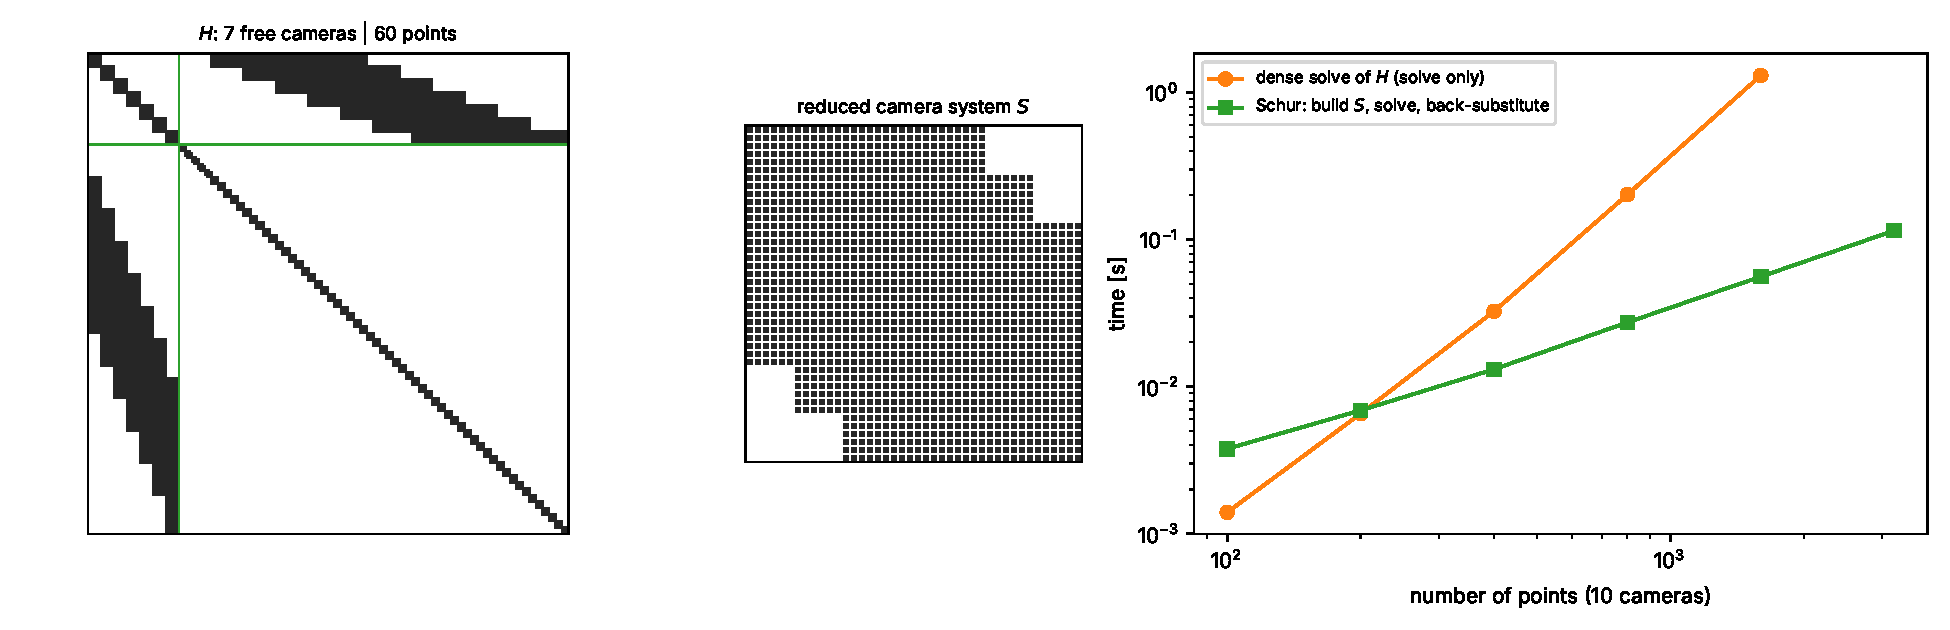
\includegraphics[width=\linewidth]{figures/ch08_structure.pdf}
\caption{Left: $H$ for 7 free cameras moving past 60 points, each seeing
40\,\% of them; the camera block (top left) is small, the point block
is a diagonal of $3\times3$ blocks, and $W$ forms the arrowhead's wings.
Middle: the reduced camera system $S$, banded because neighbouring
cameras share points. Right: time to solve the dense normal equations
(the solve alone) versus the whole Schur pipeline, 10 cameras.}
\label{fig:structure}
\end{figure}

\section{The Schur complement}

\begin{theorem}{Eliminating the points}{schurba}
Assume $V\succ0$ and $S=U-WV^{-1}W\T\succ0$. Then the solution of
$H\vect\delta=-\vect{g}$, $\vect\delta=(\vect\delta_c,\vect\delta_p)$,
is given by
\begin{align}
S\,\vect\delta_c&=-\vect{g}_c+WV^{-1}\vect{g}_p,\label{eq:rcs}\\
\vect\delta_{p}&=-V^{-1}\bigl(\vect{g}_p+W\T\vect\delta_c\bigr).
\label{eq:backsub}
\end{align}
Because $V$ is block diagonal, $V^{-1}$ costs $n$ inversions of
$3\times3$ matrices, and \eqref{eq:backsub} decouples into one $3\times3$
system per point. The same holds for the Levenberg--Marquardt system,
with $U$ and $V$ replaced by their damped versions.
\end{theorem}

\begin{proof}
The second block row of $H\vect\delta=-\vect{g}$ reads $W\T\vect\delta_c
+V\vect\delta_p=-\vect{g}_p$, which gives \eqref{eq:backsub}. The first
reads $U\vect\delta_c+W\vect\delta_p=-\vect{g}_c$; substituting
\eqref{eq:backsub}, $U\vect\delta_c-WV^{-1}\vect{g}_p-WV^{-1}W\T
\vect\delta_c=-\vect{g}_c$, which is \eqref{eq:rcs}. Conversely any
solution of \eqref{eq:rcs}--\eqref{eq:backsub} satisfies both block rows.
Damping adds $\lambda D_c$ to $U$ and $\lambda D_p$ to $V$, which keeps
both block structures.
\end{proof}

This is \cref{lem:schur} once more: $S$ is the information matrix of the
cameras after the points have been marginalised out. The direction of
the elimination matters. Eliminating the cameras first would require
inverting $U$ (cheap) but would leave a reduced system of size $3n$,
dense among all points seen by a common camera. In vision $n\gg m$, so
the points go first.

\begin{proposition}{Structure and cost of the reduced system}{rcs}
The block $S_{ik}$, $i\neq k$, equals $-\sum_jW_{ij}V_j^{-1}W_{kj}\T$,
summed over the points seen by both cameras; it is non-zero only if
cameras $i$ and $k$ share a point. If point $j$ is seen by $k_j$
cameras, forming $S$ costs $O(\sum_jk_j^2)$ small products, and solving
\eqref{eq:rcs} densely costs $O(m^3)$, against $O((m+n)^3)$ for the full
system.
\end{proposition}

\begin{proof}
$(WV^{-1}W\T)_{ik}=\sum_jW_{ij}V_j^{-1}W_{kj}\T$ since $V^{-1}$ is block
diagonal, and $W_{ij}V_j^{-1}W_{kj}\T\neq0$ requires both $W_{ij}$ and
$W_{kj}$ to be non-zero. Each point contributes one $6\times6$ product
for each ordered pair of cameras that see it.
\end{proof}

\begin{inwords}
Thousands of points, a few dozen cameras: after elimination we solve a
system whose size is set by the cameras alone, and whose sparsity is the
\emph{covisibility graph} --- which keyframes see common points. On the
right of \cref{fig:structure}, the dense solve is faster for a hundred
points, but its cost grows with the cube of the number of points, and at
1\,600 points it is already twenty times slower than the whole Schur
pipeline, which grows linearly. Large systems also solve
\eqref{eq:rcs} with a sparse Cholesky factorisation or with
preconditioned conjugate gradients; Ceres calls these
\code{SPARSE\_SCHUR} and \code{ITERATIVE\_SCHUR}.
\end{inwords}

\section{The gauge}

By \cref{prop:gauge}, the BA cost is unchanged when all cameras and
points are moved by a common rigid motion, and also by a common scale
when the observations are monocular. $H$ is then singular, with a null
space of dimension 6 (stereo) or 7 (monocular), and so is $S$. Three
remedies are in use:
\begin{itemize}[nosep]
\item \emph{fix variables}: hold the first camera constant (removing 6
  dimensions) and, for monocular BA, one more scalar, for instance the
  distance between the first two cameras;
\item \emph{add a prior} on the first pose, which makes the problem
  well posed without freezing anything;
\item \emph{let the damping handle it}: LM's $\lambda D$ makes the
  system invertible and the solver simply does not move along the null
  directions --- this works, but covariances are then meaningless.
\end{itemize}
Our solver fixes cameras listed in \code{BAProblem.fixed}; the notebook
counts the zero eigenvalues of $H$ in each case (6, 7, then 0 or 1).
Covariances depend on the choice: fixing the first camera gives every
other camera's uncertainty \emph{relative to the first one}.

\section{Uncertainty}

\begin{proposition}{Covariance from the reduced system}{bacov}
With the gauge fixed and the Laplace approximation of
\cref{prop:laplace}, the marginal covariance of the cameras is $S^{-1}$
--- so camera $i$'s is the block $(S^{-1})_{ii}$ --- and the marginal
covariance of point $j$ is
\[
\Sigma_{\vect{X}_j}=V_j^{-1}+V_j^{-1}W_{\cdot j}\T\,S^{-1}\,W_{\cdot j}
V_j^{-1},
\]
where $W_{\cdot j}$ stacks the blocks $W_{ij}$ of the cameras.
\end{proposition}

\begin{proof}
The covariance is $H^{-1}$. For a symmetric positive definite block
matrix, one checks by multiplication that
\[
\begin{pmatrix}U&W\\W\T&V\end{pmatrix}^{-1}=
\begin{pmatrix}S^{-1}&-S^{-1}WV^{-1}\\-V^{-1}W\T S^{-1}&V^{-1}+V^{-1}W\T
S^{-1}WV^{-1}\end{pmatrix}.
\]
The top-left block gives the cameras. The bottom-right block is block
diagonal plus a low-rank term; its $j$-th diagonal block is the formula
stated, since $V^{-1}$ is block diagonal.
\end{proof}

\begin{inwords}
A point's uncertainty has two parts: what its own observations say
about it with the cameras held exact ($V_j^{-1}$), plus the uncertainty
of the cameras, carried to the point through $W$. The second part is
what the VO of Chapter~\ref{ch:vo} ignored. \Cref{fig:covariance} checks
both formulas against Monte Carlo: the camera ellipses match the cloud,
and point standard deviations agree within about 30\,\% over two orders
of magnitude, the largest discrepancies being for points seen by a
single camera, where the problem is the least linear.
\end{inwords}

\begin{figure}[ht]
\centering
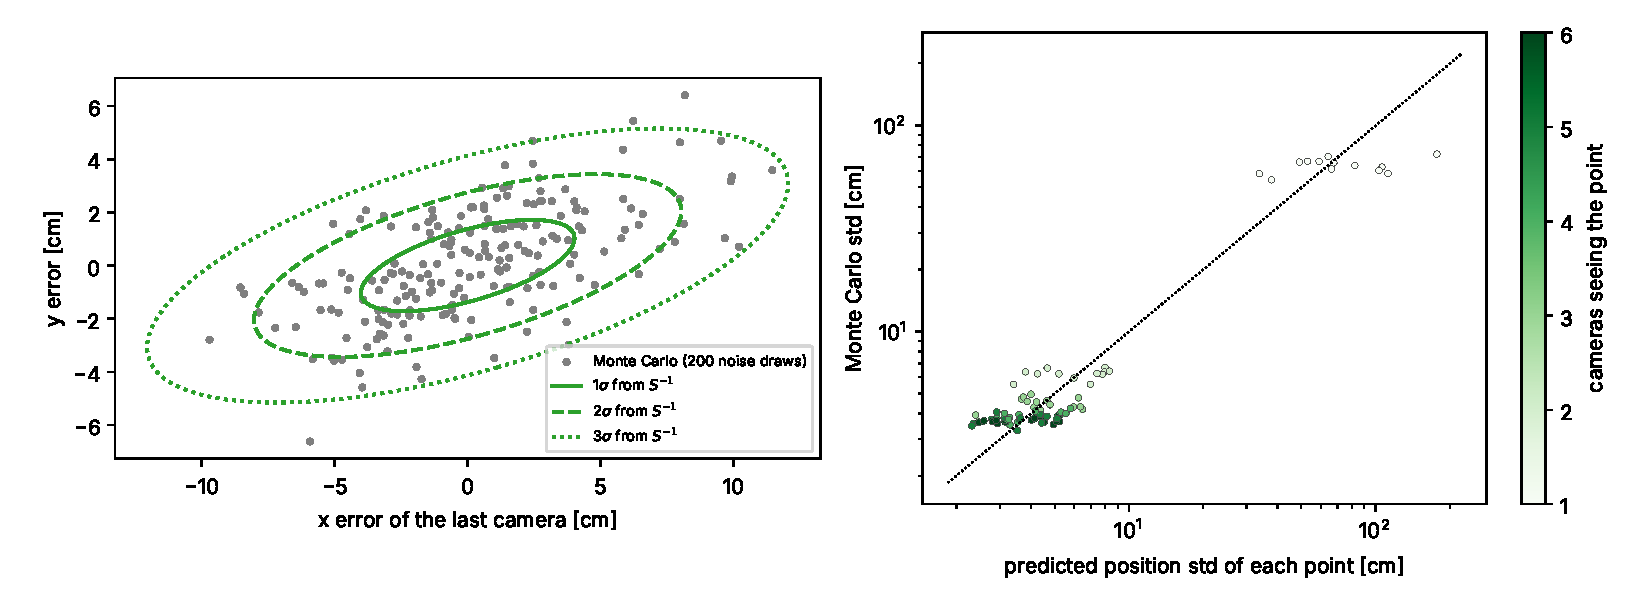
\includegraphics[width=\linewidth]{figures/ch08_covariance.pdf}
\caption{Six stereo cameras, 80 points, 0.5\,px noise, first camera
fixed; 200 noise draws. Left: position error of the last camera, with
the 1, 2 and 3$\sigma$ ellipses of $(S^{-1})_{66}$. Right: per-point
standard deviation, predicted by \cref{prop:bacov} versus Monte Carlo,
coloured by the number of cameras that see the point.}
\label{fig:covariance}
\end{figure}

\section{Local bundle adjustment}

A full BA over every keyframe is the most accurate estimate possible,
and the most expensive; it is also unnecessary at every step, since a
new keyframe only changes the recent past. A \emph{sliding-window} BA
optimises the last $N$ keyframes and the points they see, and holds
fixed the oldest keyframe of the window, which fixes the gauge and
anchors the window to the trajectory so far.

\begin{definition}{Keyframe VO with local BA}{localba}
Our \code{vslam.vo.StereoVOBA} modifies the VO of Chapter~\ref{ch:vo} in
three ways:
\begin{enumerate}[nosep]
\item map points \emph{persist} while their tracks continue: a new
  keyframe triangulates only the tracks that are not yet in the map;
\item after each new keyframe, a BA with a Cauchy kernel optimises the
  last $N=6$ keyframes and every point they observe, with all their
  stereo observations, the oldest keyframe being fixed;
\item a keyframe is created when fewer than 80\,\% (instead of 50\,\%)
  of the points of the last keyframe are still tracked, so that
  consecutive keyframes share enough points to be tied together.
\end{enumerate}
\end{definition}

The last change matters: with the Chapter~\ref{ch:vo} criterion,
consecutive keyframes share too few points, the window is poorly
connected, and the BA gains much less (in our runs, errors three to
four times larger).

\begin{figure}[ht]
\centering
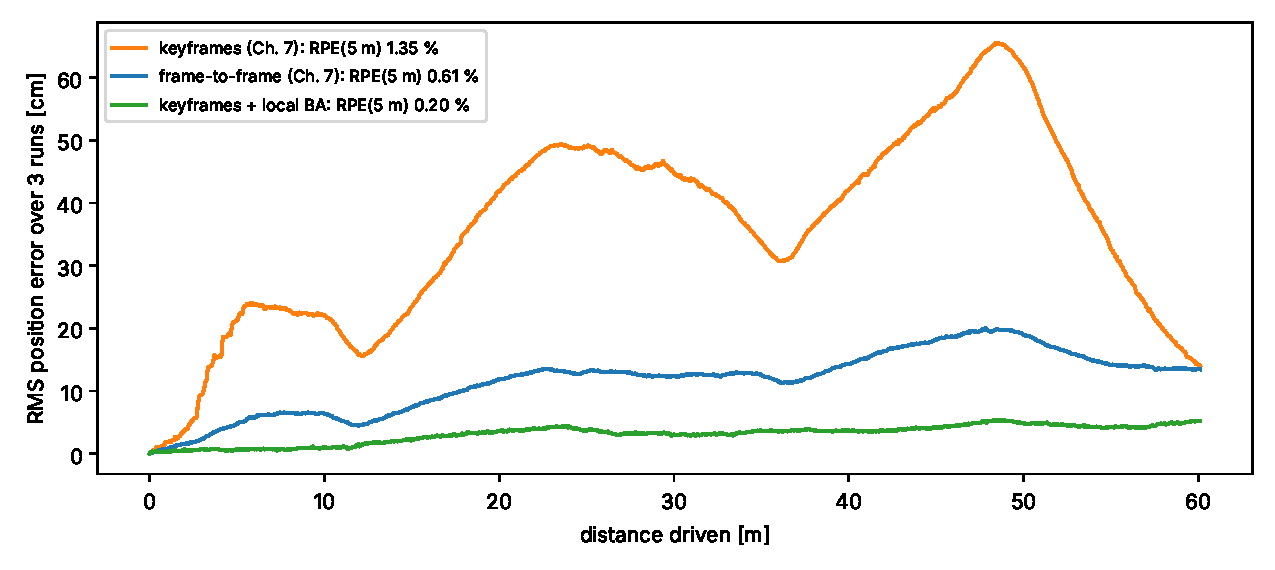
\includegraphics[width=0.9\linewidth]{figures/ch08_vo.pdf}
\caption{RMS position error along the 60\,m mowing pattern of
\cref{fig:vo}, three runs. The local BA divides the error of the
keyframe VO by more than ten and that of the frame-to-frame VO by four;
in the legend, the relative pose error over 5\,m.}
\label{fig:bavo}
\end{figure}

\Cref{fig:bavo} is the answer to Chapter~\ref{ch:vo}'s puzzle. Over three
runs of the garden: RMS error 39\,cm for the keyframe VO, 12.6\,cm for
frame-to-frame, and 3.4\,cm with the local BA; relative pose error over
5\,m 1.35\,\%, 0.61\,\% and 0.20\,\%. The same data, the same front-end,
the same localisation; the only difference is that map points are now
estimated from all the keyframes that see them, with their uncertainty
weighing in through the stereo residuals, instead of being frozen at
their first triangulation.

\begin{mower}
On the mower the BA runs in a separate thread from the tracking (as in
PTAM and ORB-SLAM): tracking must answer at frame rate, while a window
optimisation may take a few hundred milliseconds. Our Python version
needs about a minute for the 60\,m sequence instead of nine seconds;
a C++ implementation with Ceres, g2o or GTSAM is typically one to two
orders of magnitude faster, enough for a six-keyframe window in real
time.
Even at 0.2\,\%, however, the 1.7\,km of a 1\,000\,m$^2$ lawn leaves a few
metres of drift. The window is local by design: it never sees the row
mown ten minutes ago. Recognising that row --- loop closure --- is the
subject of the next two chapters.
\end{mower}

\begin{practice}[\code{vslam/ba.py}, \code{vslam/vo.py},
  \code{examples/ch08\_ba.py}, \code{notebooks/ch08\_ba.ipynb}]
\begin{center}
\begin{tabular}{@{}ll@{}}
\toprule
Code & Formula\\
\midrule
\code{BAProblem.residuals\_jacobians} & $\vect{r}_{ij}$, $A_{ij}$,
  $B_{ij}$ (vectorised)\\
\code{BAProblem.normal\_equations} & \cref{prop:arrow}\\
\code{BAProblem.schur}, \code{back\_substitute} & \cref{thm:schurba},
  \cref{prop:rcs}\\
\code{ba.solve} & LM on the reduced system, IRLS\\
\code{ba.camera\_covariance}, \code{point\_covariance} &
  \cref{prop:bacov}\\
\code{ba.dense\_system} & $H$ and $\vect{g}$, for checking\\
\code{vo.StereoVOBA} & \cref{def:localba}\\
\bottomrule
\end{tabular}
\end{center}
The tests check the Jacobian blocks against finite differences (mono
and stereo), that the Schur step equals the dense step, the dimension of
the gauge (6 for stereo, 7 for mono, minus 6 with a fixed camera), exact
convergence from a perturbed start without noise, robustness to 15\,\%
outliers, the camera covariance against Monte Carlo, and that local BA
at least halves the error of the plain VO on a 15\,m run.
\end{practice}

\section*{Further reading and C++ pointers}
\addcontentsline{toc}{section}{Further reading and C++ pointers}

B.~Triggs, P.~McLauchlan, R.~Hartley and A.~Fitzgibbon, ``Bundle
adjustment --- a modern synthesis'', 2000 (the reference); Hartley and
Zisserman, appendix~6; S.~Agarwal, N.~Snavely, S.~Seitz and R.~Szeliski,
``Bundle adjustment in the large'', ECCV 2010; G.~Klein and D.~Murray,
``Parallel tracking and mapping for small AR workspaces'' (PTAM), ISMAR
2007, for the tracking/mapping split; Mur-Artal et al.\ (ORB-SLAM) for
local BA over the covisibility graph. In C++: Ceres Solver
(\code{SPARSE\_SCHUR}), g2o (\code{BlockSolver\_6\_3}), GTSAM
(\code{GenericProjectionFactor}, \code{GenericStereoFactor}).

\FloatBarrier
\section*{Exercises}
\addcontentsline{toc}{section}{Exercises}

\begin{enumerate}[label=\textbf{8.\arabic*},ref=8.\arabic*]
\item\label{ex:8pd} Show that if $H\succ0$ then $S=U-WV^{-1}W\T\succ0$.
  (Hint: minimise the quadratic form of $H$ over $\vect\delta_p$.)
\item\label{ex:8cost} Ten keyframes, 2\,000 points, each seen by four
  keyframes. Compare, in order of magnitude, the number of operations of
  a dense Cholesky factorisation of $H$ and of the Schur pipeline.
\item\label{ex:8mono} Why can a point seen by a single stereo camera be
  estimated, while a point seen by a single monocular camera cannot?
  Answer with the rank of $V_j$.
\item\label{ex:8window} In the sliding window, the oldest keyframe is
  fixed. What would go wrong if no keyframe were fixed? And what is lost
  by fixing it?
\end{enumerate}

\subsection*{Solutions}

\textbf{8.1.} For any $\vect{x}$, the function $\vect{y}\mapsto(\vect{x},
\vect{y})\T H(\vect{x},\vect{y})=\vect{x}\T U\vect{x}+2\vect{x}\T W
\vect{y}+\vect{y}\T V\vect{y}$ is minimised at $\vect{y}=-V^{-1}W\T
\vect{x}$ ($V\succ0$ as a principal block of $H$), where its value is
$\vect{x}\T(U-WV^{-1}W\T)\vect{x}=\vect{x}\T S\vect{x}$. For
$\vect{x}\neq\vect0$ the vector $(\vect{x},\vect{y})$ is non-zero, so
this value is positive.

\textbf{8.2.} $H$ has size $6\cdot10+3\cdot2000=6060$: a dense Cholesky
costs about $6060^3/3\approx7\times10^{10}$ operations. The Schur
pipeline: $2000$ inversions of $3\times3$ blocks, $2000\times4^2=
32\,000$ products of $6\times3$ by $3\times6$ matrices (a few hundred
operations each, about $10^7$ in total), and a Cholesky factorisation of
a $60\times60$ matrix ($7\times10^4$): some four orders of magnitude
less.

\textbf{8.3.} $V_j=\sum_iB_{ij}\T B_{ij}$. A monocular observation
gives $B_{ij}$ of size $2\times3$, of rank 2 (moving the point along its
viewing ray does not change its image), so with one camera $V_j$ has
rank 2 and is singular: the depth is unknown. A stereo observation gives
a $3\times3$ $B_{ij}$ of rank 3 (the disparity measures the depth), so
$V_j\succ0$ already with one camera.

\textbf{8.4.} Without a fixed keyframe the window has a 6-dimensional
gauge freedom (\cref{prop:gauge}): $S$ is singular and, with damping,
the whole window may slide by an arbitrary small rigid motion at every
optimisation --- a drift with no cause. Fixing the oldest keyframe
removes it and ties the window to the past. The price: that keyframe's
own error is never corrected again, so drift is reduced, not abolished;
only a constraint from outside the window (a loop closure, GNSS) can
correct the past.
